%==WORKSHEET #5
\newpage
\stepcounter{handout}
\begin{exercisebox}[adjusted title= Conditionals]
With conditions, we can make things happen when special criteria are met
met. Open the aquarium project and try inserting the following into it
The \ttpy{draw} function:


\begin{lstlisting}[language=JavaScript]
if (fish1X > 500) {
    fish1X = -40;
  }

  if (fish2X < -50) {
    fish2X = 200;
  }
\end{lstlisting}

\noindent
What happens?
\end{exercisebox}

\begin{exercisebox}[adjusted title= Change direction]
By making a variable that contains the direction in which the fish swims, we can change the direction when it reaches the sides.

\begin{itemize}
\item Define a global variable \ttpy{fish1XVelocity} and set it to $1$
\item Change \ttpy{fish1X = fish1X + 1} to \ttpy{fish1X = fish1X + fish1XVelocity}
\item Remove the previous \ttpy{fish1X} condition
\item Add these conditions:
\end{itemize}


\begin{lstlisting}[language=JavaScript]
if (fish1X > 400){
    fish1XVelocity = -1
    }
if (fish1X < 0){
    fish1XVelocity = 1
    }
\end{lstlisting}
\end{exercisebox}

\begin{exercisebox}[adjusted title=Change appearance ]
Try changing the \ttpy{drawFish} function to strip the direction
with the fish as an argument and use a condition to draw the fins and
eyes differently depending on which direction the fish is swimming.

\begin{minipage}{0.60\linewidth}
\begin{lstlisting}[language=JavaScript]
function drawFish(x, y, eyeSize, velocity){
    ... daw body ...

    # Swim to the right
    if (velocity >= 0){
        ...draw fins and eyes ...
        }

    # Swim to the left
    if (velocity < 0){
        ...draw fins and eyes ...
        }
}
\end{lstlisting}

\end{minipage}
\begin{minipage}{0.40\linewidth}
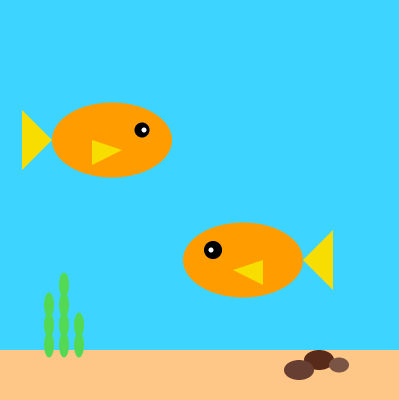
\includegraphics[width=0.70\textwidth]{illustrationer/fisk-begge-retninger.png}
\end{minipage}
~
\end{exercisebox}


\begin{exercisebox}[adjusted title=Finish the aquarium project ]
Now, we are almost done with the aquarium project. Add, if necessary, more elements. E.g. bubbles that emerge from the bottom and swim towards the surface.
\end{exercisebox}

%\newpage
%
\begin{exercisebox}[adjusted title=More exercises about conditions]
Open the Green City project and do the following:
\begin{itemize}
\item Make the cloud move back to the start and pass by again and
 again, each time it hits the edge
\item Make the car turn over at both ends.
\end{itemize}
\tcbsubtitle{Tasks:}
The car must stop when the battery is empty
 \begin{itemize}
 \item Define a global variable \ttpy{carBattery} and set it to 100
 \item Decrease it by 0.1 each time \ttpy{draw} is called
 \item Display the battery status using the \ttpy{text(string, x, y)} function.
 Remember to convert the number to a string using \ttpy{str()}.
 \item If the battery is empty (\ttpy{<= 0}) the car must stop (set velocity to 0)
 \end{itemize}
Add a \ttpy{keyPressed()} function and make it possible to charge the electric car when you press 'C':
 \begin{itemize}
 \item Add \ttpy{0.3} to \ttpy{carBattery} every time 'C' is pressed on the keyboard
 \item If \ttpy{carBattery} exceeds 100, set it to 100 so you can't charge more than 100\%
 \end{itemize}
\end{exercisebox}


\begin{exercisebox}[adjusted title= Changing wind speed]
The variable \ttpy{frameCount} counts how many times \ttpy{draw} is
run since the program started. Enter this in the draw function i
the electric car project:


\begin{lstlisting}[language=JavaScript]
fill(0, 0, 0);
text(frameCount, 350, 20):
if (frameCount % 60 == 0){
    print(frameCount)
    }
\end{lstlisting}

%new stuff


\noindent
Since \ttpy{draw} is executed at \textit{60 frames per second}, will
The \ttpy{print} function will be executed every second.

\vspace{2mm}
\noindent
We can also use that in the electric car project to update
the wind speed every second.
 \begin{itemize}
 \item Create a global windSpeed ​​variable
 \item Update windSpeed ​​with a new random value every second
 \item Display the wind speed using \ttpy{text()}
 \end{itemize}
% \item Turn the power plant on and off
 \begin{itemize}
 \item Create a global variable \ttpy{powerplantOn}
 \item Make it possible to turn the power plant on and off with a press of 'p'
 \item Draw clouds of smoke over the power plant when it is on
 \item Create a variable \ttpy{co2emission} and add a bit as long
 the power plant is on. Display the value with \ttpy{text()}
 \end{itemize}
 \end{exercisebox}


\begin{exercisebox}[adjusted title= Introduction to Sounds]
In this small worksheet, we will add sound files to make sound effects!

\begin{enumerate}
\item First check reference https://p5js.org/reference/p5.MediaElement/play/
\item Then download the sound files from ABASALON 
\item Also check out the sound sketch also uploaded
\item Create a new file and names  \ttpy{sound01}

\end{enumerate}


\begin{lstlisting}[language=JavaScript]
function preload() {
  // Load the sound files before the program starts
   // Load the first sound file (e.g., a music track or sound effect)
  sound = loadSound('sound.mp3'); 
  // Load the second sound file (e.g., a ball tap sound)
  sound1 = loadSound('balltap.wav');  
}

function setup() {
  // Setup the canvas size
  createCanvas(400, 400);  // Create a canvas of 400x400 pixels
}

function draw() {
  // Draw the background and instructions
  background(220);  // Set the background color to light grey (RGB value: 220)
  // Align text to the center horizontally and vertically
  textAlign(CENTER, CENTER);  
  textSize(24);  // Set the text size to 24 pixels
  // Display the instructions in the center of the canvas
  text('Press "S" or "A" to play sound', width / 2, height / 2);  
}

function keyPressed() {
  // Detect key presses and play the corresponding sound
  if (key === 's' || key === 'S') {
    // Play the first sound when the 'S' key is pressed (case insensitive)
    sound.play();
  }
  if (key === 'a' || key === 'A') {
    // Play the second sound when the 'A' key is pressed (case insensitive)
    sound1.play();
  }
}
\end{lstlisting}

\textbf{Descrptions}

\begin{itemize}
    \item \textbf{`preload()` function}: Loads the sound files into memory before the sketch starts. This ensures that the sounds are ready to be played when triggered.
    \item \textbf{`setup()` function}: Sets up the canvas where the sketch will be displayed, specifying its size (400x400 pixels).
    \item \textbf{`draw()` function}: Continuously runs in a loop, updating the background color and displaying the instruction text centered on the canvas.
    \item \textbf{`keyPressed()` function}: Listens for specific key presses ('S' or 'A') and plays the corresponding sound when either key is pressed.
\end{itemize}

\end{exercisebox}

%With \ttpy{for loops}, we can avoid duplicated code and iteratively perform an operation, such as drawing 3 circles on a screen.
%Start a new project and insert the following code:
%
%\begin{lstlisting}[language=JavaScript]
%// Initialize Lists
%let xs = [30, 50, 70, 90, 110, 130];
%let ys = [30, 50, 70, 90, 110, 130];
%
%function setup() {
%  createCanvas(400, 400);
%  background(0);
%}
%
%function drawCircle(x, y) {
%  noStroke();
%  bubble_R = random(256);
%  bubble_G = random(256);
%  bubble_B = random(256);
%  fill(bubble_R, bubble_G, bubble_B);
%  circle(x, y, 25);
%}
%
%function draw() {
%  for (var i = 0; i < xs.length; i++) {
%    drawCircle(xs[i], ys[i]);
%  }
%}
%\end{lstlisting}
%
%What happens when you run the code? Explain here how a loop produces the result, and give yourself time to understand the logic.
%
%\end{exercisebox}
%
%\begin{exercisebox}[adjusted title= More with Lists and For Loops]
%The following code snippet has a few changes: We now use a loop to generate our list! Paste the code into a new project and consider the differences in the various loops.
%
%\begin{lstlisting}[language=JavaScript]
%// Initialize Lists
%let circleList = [];
%
%function setup() {
%  createCanvas(400, 400);
%  background(0);
%}
%
%function drawCircle(x, y) {
%  stroke(255, 255, 255);
%  noStroke();
%  bubble_R =random(255);
%  bubble_G =random(255);
%  bubble_B =random(255);
%  fill(bubble_R, bubble_G, bubble_B);
%  circle(x, 200, 50);
%}
%
%function createCircleList(n) {
%  for (var i=0; i < n; i++) {
%    append(circleList, i*60);
%  }
%}
%
%function draw() {
%  createCircleList(10);
%  for (var i = 0; i < circleList.length; i++) {
%    drawCircle(i);
%  }
%}
%\end{lstlisting}
%
%\noindent
%
%\vspace{2mm}
%\noindent
%
%\begin{itemize}
%  \item Use loops and lists to move your fish or make more fish in different locations. Plus in Green City if you want.
%\end{itemize}
%\end{exercisebox}